\chapter{Analisi ammortizzata}

\index{analisi ammortizzata}

La complessità computazionale di un algoritmo
è spesso facile da analizzare, 
esaminando la struttura dell'algoritmo:
quanti cicli contiene e quante volte 
questi cicli sono eseguiti.
Comunque non sempre un'analisi diretta
da una stima significativa dell'efficienza di un algoritmo.

L'\key{analisi ammortizzata} può essere usata per analizzare
algoritmi che contengono operazioni la 
cui complessità varia nelle varie esecuzioni.
L'idea è di stimare il tempo totale usato
da tutte le operazioni eseguite dall'algoritmo,
al posto di concentrarsi sulle singole operazioni.

\section{Metodo dei due puntatori}

\index{metodo dei due puntatori}

Nel \key{metodo dei due puntatori},
vengono utilizzati due puntatori, o indici, 
per iterare attraverso i valori di un array.
Entrambi i puntatori possono muoversi in una direzione soltanto,
il chè assicura che l'algoritmo sarà molto efficiente.
Adesso si discuteranno due problemi in cui
può essere utilizzato questo metodo.

\subsubsection{Somma di un sottovettore}

Come primo esempio,
si consideri un problema dove,
dato un vettore composto da $n$ interi positivi
e una somma obiettivo $x$,
si voglia trovare un sottovettore la cui somma sia
esattamente $x$, oppure comunicare che questa cosa non è possibile.

Per esempio, l'array
\begin{center}
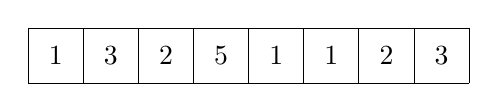
\begin{tikzpicture}[scale=0.7]
\draw (0,0) grid (8,1);

\node at (0.5,0.5) {$1$};
\node at (1.5,0.5) {$3$};
\node at (2.5,0.5) {$2$};
\node at (3.5,0.5) {$5$};
\node at (4.5,0.5) {$1$};
\node at (5.5,0.5) {$1$};
\node at (6.5,0.5) {$2$};
\node at (7.5,0.5) {$3$};
\end{tikzpicture}
\end{center}
contiene un sottovettore la cui somma è 8:
\begin{center}
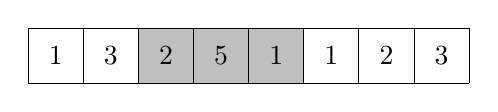
\begin{tikzpicture}[scale=0.7]
\fill[color=lightgray] (2,0) rectangle (5,1);
\draw (0,0) grid (8,1);

\node at (0.5,0.5) {$1$};
\node at (1.5,0.5) {$3$};
\node at (2.5,0.5) {$2$};
\node at (3.5,0.5) {$5$};
\node at (4.5,0.5) {$1$};
\node at (5.5,0.5) {$1$};
\node at (6.5,0.5) {$2$};
\node at (7.5,0.5) {$3$};
\end{tikzpicture}
\end{center}

Questo problema può essere risolto in tempo
$O(n)$ usando il metodo dei due puntatori.
L'idea è quella di avere un puntatore al primo e 
l'altro all'ultimo elemento del sottovettore cercato.
A ogni passaggio, il puntatore di sinistra si muoverà 
di un passo a destra e il puntatore destro si muoverà a destra
fino a quando la somma del sottovettore risultante sia al massimo $x$.
Se la somma diventa esattamente $x$,
allora è stata trovata una soluzione.

Come esempio si consideri questo array e 
la somma obiettivo sia $x=8$:
\begin{center}
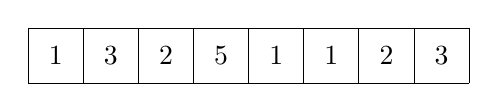
\begin{tikzpicture}[scale=0.7]
\draw (0,0) grid (8,1);

\node at (0.5,0.5) {$1$};
\node at (1.5,0.5) {$3$};
\node at (2.5,0.5) {$2$};
\node at (3.5,0.5) {$5$};
\node at (4.5,0.5) {$1$};
\node at (5.5,0.5) {$1$};
\node at (6.5,0.5) {$2$};
\node at (7.5,0.5) {$3$};
\end{tikzpicture}
\end{center}

All'inizio il sottovettore contiene i valori
1, 3 e 3, la cui somma è 6 (il 5 non viene incluso adesso
perchè porterebbe la somma a un valore maggiore di 8):

\begin{center}
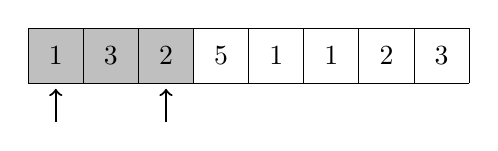
\begin{tikzpicture}[scale=0.7]
\fill[color=lightgray] (0,0) rectangle (3,1);
\draw (0,0) grid (8,1);

\node at (0.5,0.5) {$1$};
\node at (1.5,0.5) {$3$};
\node at (2.5,0.5) {$2$};
\node at (3.5,0.5) {$5$};
\node at (4.5,0.5) {$1$};
\node at (5.5,0.5) {$1$};
\node at (6.5,0.5) {$2$};
\node at (7.5,0.5) {$3$};

\draw[thick,->] (0.5,-0.7) -- (0.5,-0.1);
\draw[thick,->] (2.5,-0.7) -- (2.5,-0.1);
\end{tikzpicture}
\end{center}

Poi il puntatore di sinistra si muove di una posizione a destra
e ancora il puntatore destro sta fermo, altrimenti la somma
eccederebbe il valore di $x$.

\begin{center}
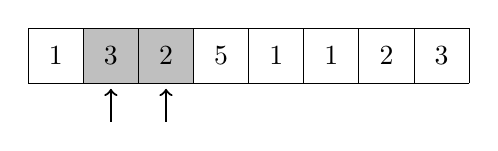
\begin{tikzpicture}[scale=0.7]
\fill[color=lightgray] (1,0) rectangle (3,1);
\draw (0,0) grid (8,1);

\node at (0.5,0.5) {$1$};
\node at (1.5,0.5) {$3$};
\node at (2.5,0.5) {$2$};
\node at (3.5,0.5) {$5$};
\node at (4.5,0.5) {$1$};
\node at (5.5,0.5) {$1$};
\node at (6.5,0.5) {$2$};
\node at (7.5,0.5) {$3$};

\draw[thick,->] (1.5,-0.7) -- (1.5,-0.1);
\draw[thick,->] (2.5,-0.7) -- (2.5,-0.1);
\end{tikzpicture}
\end{center}

Il puntatore di sinistra si muove ancora di un passo, 
e questa volta il puntatore di destra si muove di 3 passi
a destra.
Siccome adesso la somma è esattamente 8 ($2+5+1$),
la soluzione cercata è stata trovata.

\begin{center}
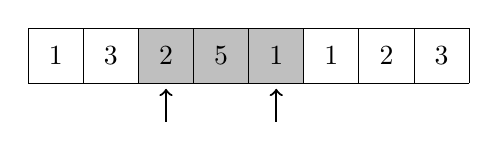
\begin{tikzpicture}[scale=0.7]
\fill[color=lightgray] (2,0) rectangle (5,1);
\draw (0,0) grid (8,1);

\node at (0.5,0.5) {$1$};
\node at (1.5,0.5) {$3$};
\node at (2.5,0.5) {$2$};
\node at (3.5,0.5) {$5$};
\node at (4.5,0.5) {$1$};
\node at (5.5,0.5) {$1$};
\node at (6.5,0.5) {$2$};
\node at (7.5,0.5) {$3$};

\draw[thick,->] (2.5,-0.7) -- (2.5,-0.1);
\draw[thick,->] (4.5,-0.7) -- (4.5,-0.1);
\end{tikzpicture}
\end{center}

Il tempo di esecuzione di questo algoritmo dipende
dal numero di spostamenti che compie il puntatore
di destra a ogni passaggio.
Nonostante non ci sia un limite superiore significativo 
al numero di spostamenti che può compiere a ogni singolo
passaggio, si può comunque vedere che il puntatore farà al 
massimo \emph{un totale di }
$O(n)$ passaggi durante l'algoritmo,
poichè si muove sempre solo a destra.

Poichè sia il puntatore di sinistra che quello di destra
si muovono di $O(n)$ passi durante l'esecuzione dell'algoritmo,
la complessità computazionale è di tipo $O(n)$.

\subsubsection{2SUM problem}

\index{2SUM problem}

Another problem that can be solved using
the two pointers method is the following problem,
also known as the \key{2SUM problem}:
given an array of $n$ numbers and
a target sum $x$, find
two array values such that their sum is $x$,
or report that no such values exist.

To solve the problem, we first
sort the array values in increasing order.
After that, we iterate through the array using
two pointers.
The left pointer starts at the first value
and moves one step to the right on each turn.
The right pointer begins at the last value
and always moves to the left until the sum of the
left and right value is at most $x$.
If the sum is exactly $x$,
a solution has been found.

For example, consider the following array
and a target sum $x=12$:
\begin{center}
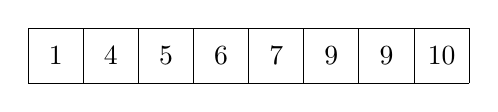
\begin{tikzpicture}[scale=0.7]
\draw (0,0) grid (8,1);

\node at (0.5,0.5) {$1$};
\node at (1.5,0.5) {$4$};
\node at (2.5,0.5) {$5$};
\node at (3.5,0.5) {$6$};
\node at (4.5,0.5) {$7$};
\node at (5.5,0.5) {$9$};
\node at (6.5,0.5) {$9$};
\node at (7.5,0.5) {$10$};
\end{tikzpicture}
\end{center}

The initial positions of the pointers
are as follows.
The sum of the values is $1+10=11$
that is smaller than $x$.

\begin{center}
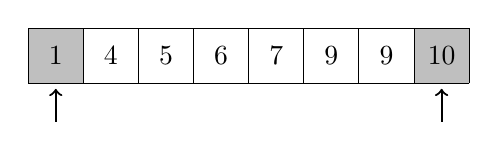
\begin{tikzpicture}[scale=0.7]
\fill[color=lightgray] (0,0) rectangle (1,1);
\fill[color=lightgray] (7,0) rectangle (8,1);
\draw (0,0) grid (8,1);

\node at (0.5,0.5) {$1$};
\node at (1.5,0.5) {$4$};
\node at (2.5,0.5) {$5$};
\node at (3.5,0.5) {$6$};
\node at (4.5,0.5) {$7$};
\node at (5.5,0.5) {$9$};
\node at (6.5,0.5) {$9$};
\node at (7.5,0.5) {$10$};

\draw[thick,->] (0.5,-0.7) -- (0.5,-0.1);
\draw[thick,->] (7.5,-0.7) -- (7.5,-0.1);
\end{tikzpicture}
\end{center}

Then the left pointer moves one step to the right.
The right pointer moves three steps to the left,
and the sum becomes $4+7=11$.

\begin{center}
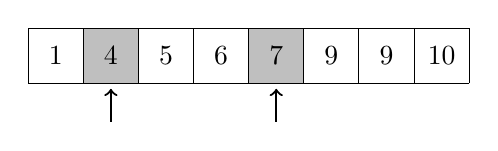
\begin{tikzpicture}[scale=0.7]
\fill[color=lightgray] (1,0) rectangle (2,1);
\fill[color=lightgray] (4,0) rectangle (5,1);
\draw (0,0) grid (8,1);

\node at (0.5,0.5) {$1$};
\node at (1.5,0.5) {$4$};
\node at (2.5,0.5) {$5$};
\node at (3.5,0.5) {$6$};
\node at (4.5,0.5) {$7$};
\node at (5.5,0.5) {$9$};
\node at (6.5,0.5) {$9$};
\node at (7.5,0.5) {$10$};

\draw[thick,->] (1.5,-0.7) -- (1.5,-0.1);
\draw[thick,->] (4.5,-0.7) -- (4.5,-0.1);
\end{tikzpicture}
\end{center}

After this, the left pointer moves one step to the right again.
The right pointer does not move, and a solution
$5+7=12$ has been found.

\begin{center}
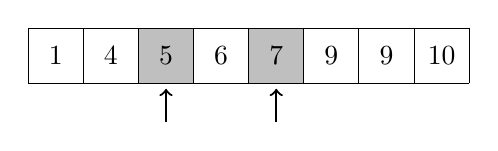
\begin{tikzpicture}[scale=0.7]
\fill[color=lightgray] (2,0) rectangle (3,1);
\fill[color=lightgray] (4,0) rectangle (5,1);
\draw (0,0) grid (8,1);

\node at (0.5,0.5) {$1$};
\node at (1.5,0.5) {$4$};
\node at (2.5,0.5) {$5$};
\node at (3.5,0.5) {$6$};
\node at (4.5,0.5) {$7$};
\node at (5.5,0.5) {$9$};
\node at (6.5,0.5) {$9$};
\node at (7.5,0.5) {$10$};

\draw[thick,->] (2.5,-0.7) -- (2.5,-0.1);
\draw[thick,->] (4.5,-0.7) -- (4.5,-0.1);
\end{tikzpicture}
\end{center}

The running time of the algorithm is
$O(n \log n)$, because it first sorts
the array in $O(n \log n)$ time,
and then both pointers move $O(n)$ steps.

Note that it is possible to solve the problem
in another way in $O(n \log n)$ time using binary search.
In such a solution, we iterate through the array
and for each array value, we try to find another
value that yields the sum $x$.
This can be done by performing $n$ binary searches,
each of which takes $O(\log n)$ time.

\index{3SUM problem}
A more difficult problem is 
the \key{3SUM problem} that asks to
find \emph{three} array values
whose sum is $x$.
Using the idea of the above algorithm,
this problem can be solved in $O(n^2)$ time\footnote{For a long time,
it was thought that solving
the 3SUM problem more efficiently than in $O(n^2)$ time
would not be possible.
However, in 2014, it turned out \cite{gro14}
that this is not the case.}.
Can you see how?

\section{Nearest smaller elements}

\index{nearest smaller elements}

Amortized analysis is often used to
estimate the number of operations
performed on a data structure.
The operations may be distributed unevenly so
that most operations occur during a
certain phase of the algorithm, but the total
number of the operations is limited.

As an example, consider the problem
of finding for each array element
the \key{nearest smaller element}, i.e.,
the first smaller element that precedes the element
in the array.
It is possible that no such element exists,
in which case the algorithm should report this.
Next we will see how the problem can be
efficiently solved using a stack structure.

We go through the array from left to right
and maintain a stack of array elements.
At each array position, we remove elements from the stack
until the top element is smaller than the
current element, or the stack is empty.
Then, we report that the top element is
the nearest smaller element of the current element,
or if the stack is empty, there is no such element.
Finally, we add the current element to the stack.

As an example, consider the following array:
\begin{center}
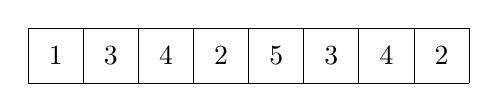
\begin{tikzpicture}[scale=0.7]
\draw (0,0) grid (8,1);

\node at (0.5,0.5) {$1$};
\node at (1.5,0.5) {$3$};
\node at (2.5,0.5) {$4$};
\node at (3.5,0.5) {$2$};
\node at (4.5,0.5) {$5$};
\node at (5.5,0.5) {$3$};
\node at (6.5,0.5) {$4$};
\node at (7.5,0.5) {$2$};
\end{tikzpicture}
\end{center}

First, the elements 1, 3 and 4 are added to the stack,
because each element is larger than the previous element.
Thus, the nearest smaller element of 4 is 3,
and the nearest smaller element of 3 is 1.
\begin{center}
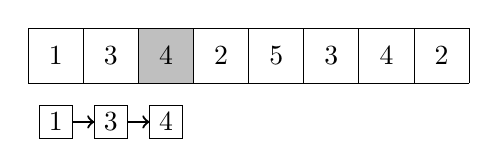
\begin{tikzpicture}[scale=0.7]
\fill[color=lightgray] (2,0) rectangle (3,1);
\draw (0,0) grid (8,1);

\node at (0.5,0.5) {$1$};
\node at (1.5,0.5) {$3$};
\node at (2.5,0.5) {$4$};
\node at (3.5,0.5) {$2$};
\node at (4.5,0.5) {$5$};
\node at (5.5,0.5) {$3$};
\node at (6.5,0.5) {$4$};
\node at (7.5,0.5) {$2$};

\draw (0.2,0.2-1.2) rectangle (0.8,0.8-1.2);
\draw (1.2,0.2-1.2) rectangle (1.8,0.8-1.2);
\draw (2.2,0.2-1.2) rectangle (2.8,0.8-1.2);

\node at (0.5,0.5-1.2) {$1$};
\node at (1.5,0.5-1.2) {$3$};
\node at (2.5,0.5-1.2) {$4$};

\draw[->,thick] (0.8,0.5-1.2) -- (1.2,0.5-1.2);
\draw[->,thick] (1.8,0.5-1.2) -- (2.2,0.5-1.2);
\end{tikzpicture}
\end{center}

The next element 2 is smaller than the two top
elements in the stack.
Thus, the elements 3 and 4 are removed from the stack,
and then the element 2 is added to the stack.
Its nearest smaller element is 1:
\begin{center}
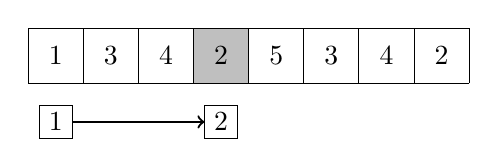
\begin{tikzpicture}[scale=0.7]
\fill[color=lightgray] (3,0) rectangle (4,1);
\draw (0,0) grid (8,1);

\node at (0.5,0.5) {$1$};
\node at (1.5,0.5) {$3$};
\node at (2.5,0.5) {$4$};
\node at (3.5,0.5) {$2$};
\node at (4.5,0.5) {$5$};
\node at (5.5,0.5) {$3$};
\node at (6.5,0.5) {$4$};
\node at (7.5,0.5) {$2$};

\draw (0.2,0.2-1.2) rectangle (0.8,0.8-1.2);
\draw (3.2,0.2-1.2) rectangle (3.8,0.8-1.2);

\node at (0.5,0.5-1.2) {$1$};
\node at (3.5,0.5-1.2) {$2$};

\draw[->,thick] (0.8,0.5-1.2) -- (3.2,0.5-1.2);
\end{tikzpicture}
\end{center}

Then, the element 5 is larger than the element 2,
so it will be added to the stack, and
its nearest smaller element is 2:
\begin{center}
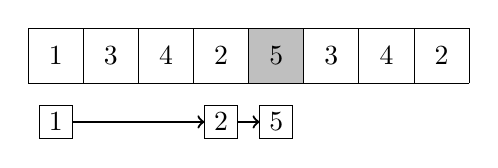
\begin{tikzpicture}[scale=0.7]
\fill[color=lightgray] (4,0) rectangle (5,1);
\draw (0,0) grid (8,1);

\node at (0.5,0.5) {$1$};
\node at (1.5,0.5) {$3$};
\node at (2.5,0.5) {$4$};
\node at (3.5,0.5) {$2$};
\node at (4.5,0.5) {$5$};
\node at (5.5,0.5) {$3$};
\node at (6.5,0.5) {$4$};
\node at (7.5,0.5) {$2$};

\draw (0.2,0.2-1.2) rectangle (0.8,0.8-1.2);
\draw (3.2,0.2-1.2) rectangle (3.8,0.8-1.2);
\draw (4.2,0.2-1.2) rectangle (4.8,0.8-1.2);

\node at (0.5,0.5-1.2) {$1$};
\node at (3.5,0.5-1.2) {$2$};
\node at (4.5,0.5-1.2) {$5$};

\draw[->,thick] (0.8,0.5-1.2) -- (3.2,0.5-1.2);
\draw[->,thick] (3.8,0.5-1.2) -- (4.2,0.5-1.2);
\end{tikzpicture}
\end{center}

After this, the element 5 is removed from the stack
and the elements 3 and 4 are added to the stack:
\begin{center}
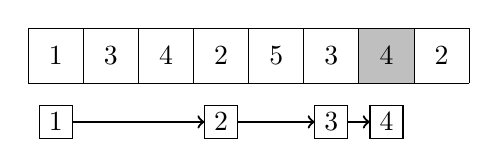
\begin{tikzpicture}[scale=0.7]
\fill[color=lightgray] (6,0) rectangle (7,1);
\draw (0,0) grid (8,1);

\node at (0.5,0.5) {$1$};
\node at (1.5,0.5) {$3$};
\node at (2.5,0.5) {$4$};
\node at (3.5,0.5) {$2$};
\node at (4.5,0.5) {$5$};
\node at (5.5,0.5) {$3$};
\node at (6.5,0.5) {$4$};
\node at (7.5,0.5) {$2$};

\draw (0.2,0.2-1.2) rectangle (0.8,0.8-1.2);
\draw (3.2,0.2-1.2) rectangle (3.8,0.8-1.2);
\draw (5.2,0.2-1.2) rectangle (5.8,0.8-1.2);
\draw (6.2,0.2-1.2) rectangle (6.8,0.8-1.2);

\node at (0.5,0.5-1.2) {$1$};
\node at (3.5,0.5-1.2) {$2$};
\node at (5.5,0.5-1.2) {$3$};
\node at (6.5,0.5-1.2) {$4$};

\draw[->,thick] (0.8,0.5-1.2) -- (3.2,0.5-1.2);
\draw[->,thick] (3.8,0.5-1.2) -- (5.2,0.5-1.2);
\draw[->,thick] (5.8,0.5-1.2) -- (6.2,0.5-1.2);
\end{tikzpicture}
\end{center}

Finally, all elements except 1 are removed
from the stack and the last element 2
is added to the stack:

\begin{center}
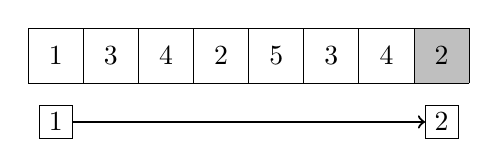
\begin{tikzpicture}[scale=0.7]
\fill[color=lightgray] (7,0) rectangle (8,1);
\draw (0,0) grid (8,1);

\node at (0.5,0.5) {$1$};
\node at (1.5,0.5) {$3$};
\node at (2.5,0.5) {$4$};
\node at (3.5,0.5) {$2$};
\node at (4.5,0.5) {$5$};
\node at (5.5,0.5) {$3$};
\node at (6.5,0.5) {$4$};
\node at (7.5,0.5) {$2$};

\draw (0.2,0.2-1.2) rectangle (0.8,0.8-1.2);
\draw (7.2,0.2-1.2) rectangle (7.8,0.8-1.2);

\node at (0.5,0.5-1.2) {$1$};
\node at (7.5,0.5-1.2) {$2$};

\draw[->,thick] (0.8,0.5-1.2) -- (7.2,0.5-1.2);
\end{tikzpicture}
\end{center}

The efficiency of the algorithm depends on
the total number of stack operations.
If the current element is larger than
the top element in the stack, it is directly
added to the stack, which is efficient.
However, sometimes the stack can contain several
larger elements and it takes time to remove them.
Still, each element is added \emph{exactly once} to the stack
and removed \emph{at most once} from the stack.
Thus, each element causes $O(1)$ stack operations,
and the algorithm works in $O(n)$ time.

\section{Sliding window minimum}

\index{sliding window}
\index{sliding window minimum}

A \key{sliding window} is a constant-size subarray
that moves from left to right through the array.
At each window position,
we want to calculate some information
about the elements inside the window.
In this section, we focus on the problem
of maintaining the \key{sliding window minimum},
which means that
we should report the smallest value inside each window.

The sliding window minimum can be calculated
using a similar idea that we used to calculate
the nearest smaller elements.
We maintain a queue
where each element is larger than
the previous element,
and the first element
always corresponds to the minimum element inside the window.
After each window move,
we remove elements from the end of the queue
until the last queue element
is smaller than the new window element,
or the queue becomes empty.
We also remove the first queue element
if it is not inside the window anymore.
Finally, we add the new window element
to the end of the queue.

As an example, consider the following array:

\begin{center}
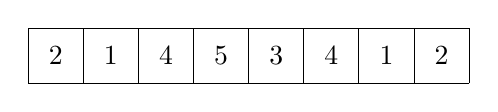
\begin{tikzpicture}[scale=0.7]
\draw (0,0) grid (8,1);

\node at (0.5,0.5) {$2$};
\node at (1.5,0.5) {$1$};
\node at (2.5,0.5) {$4$};
\node at (3.5,0.5) {$5$};
\node at (4.5,0.5) {$3$};
\node at (5.5,0.5) {$4$};
\node at (6.5,0.5) {$1$};
\node at (7.5,0.5) {$2$};
\end{tikzpicture}
\end{center}

Suppose that the size of the sliding window is 4.
At the first window position, the smallest value is 1:
\begin{center}
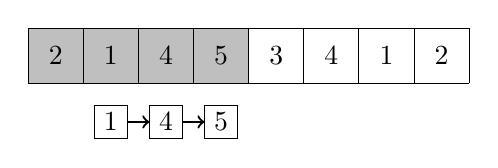
\begin{tikzpicture}[scale=0.7]
\fill[color=lightgray] (0,0) rectangle (4,1);
\draw (0,0) grid (8,1);

\node at (0.5,0.5) {$2$};
\node at (1.5,0.5) {$1$};
\node at (2.5,0.5) {$4$};
\node at (3.5,0.5) {$5$};
\node at (4.5,0.5) {$3$};
\node at (5.5,0.5) {$4$};
\node at (6.5,0.5) {$1$};
\node at (7.5,0.5) {$2$};

\draw (1.2,0.2-1.2) rectangle (1.8,0.8-1.2);
\draw (2.2,0.2-1.2) rectangle (2.8,0.8-1.2);
\draw (3.2,0.2-1.2) rectangle (3.8,0.8-1.2);

\node at (1.5,0.5-1.2) {$1$};
\node at (2.5,0.5-1.2) {$4$};
\node at (3.5,0.5-1.2) {$5$};

\draw[->,thick] (1.8,0.5-1.2) -- (2.2,0.5-1.2);
\draw[->,thick] (2.8,0.5-1.2) -- (3.2,0.5-1.2);
\end{tikzpicture}
\end{center}

Then the window moves one step right.
The new element 3 is smaller than the elements
4 and 5 in the queue, so the elements 4 and 5
are removed from the queue
and the element 3 is added to the queue.
The smallest value is still 1.
\begin{center}
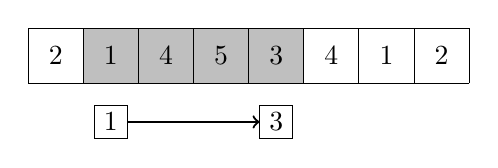
\begin{tikzpicture}[scale=0.7]
\fill[color=lightgray] (1,0) rectangle (5,1);
\draw (0,0) grid (8,1);

\node at (0.5,0.5) {$2$};
\node at (1.5,0.5) {$1$};
\node at (2.5,0.5) {$4$};
\node at (3.5,0.5) {$5$};
\node at (4.5,0.5) {$3$};
\node at (5.5,0.5) {$4$};
\node at (6.5,0.5) {$1$};
\node at (7.5,0.5) {$2$};

\draw (1.2,0.2-1.2) rectangle (1.8,0.8-1.2);
\draw (4.2,0.2-1.2) rectangle (4.8,0.8-1.2);

\node at (1.5,0.5-1.2) {$1$};
\node at (4.5,0.5-1.2) {$3$};

\draw[->,thick] (1.8,0.5-1.2) -- (4.2,0.5-1.2);
\end{tikzpicture}
\end{center}

After this, the window moves again,
and the smallest element 1
does not belong to the window anymore.
Thus, it is removed from the queue and the smallest
value is now 3. Also the new element 4
is added to the queue.
\begin{center}
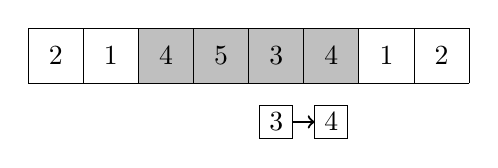
\begin{tikzpicture}[scale=0.7]
\fill[color=lightgray] (2,0) rectangle (6,1);
\draw (0,0) grid (8,1);

\node at (0.5,0.5) {$2$};
\node at (1.5,0.5) {$1$};
\node at (2.5,0.5) {$4$};
\node at (3.5,0.5) {$5$};
\node at (4.5,0.5) {$3$};
\node at (5.5,0.5) {$4$};
\node at (6.5,0.5) {$1$};
\node at (7.5,0.5) {$2$};

\draw (4.2,0.2-1.2) rectangle (4.8,0.8-1.2);
\draw (5.2,0.2-1.2) rectangle (5.8,0.8-1.2);

\node at (4.5,0.5-1.2) {$3$};
\node at (5.5,0.5-1.2) {$4$};

\draw[->,thick] (4.8,0.5-1.2) -- (5.2,0.5-1.2);
\end{tikzpicture}
\end{center}

The next new element 1 is smaller than all elements
in the queue.
Thus, all elements are removed from the queue
and it will only contain the element 1:
\begin{center}
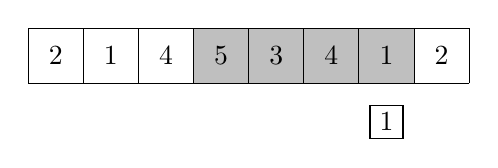
\begin{tikzpicture}[scale=0.7]
\fill[color=lightgray] (3,0) rectangle (7,1);
\draw (0,0) grid (8,1);

\node at (0.5,0.5) {$2$};
\node at (1.5,0.5) {$1$};
\node at (2.5,0.5) {$4$};
\node at (3.5,0.5) {$5$};
\node at (4.5,0.5) {$3$};
\node at (5.5,0.5) {$4$};
\node at (6.5,0.5) {$1$};
\node at (7.5,0.5) {$2$};

\draw (6.2,0.2-1.2) rectangle (6.8,0.8-1.2);

\node at (6.5,0.5-1.2) {$1$};
\end{tikzpicture}
\end{center}

Finally the window reaches its last position.
The element 2 is added to the queue,
but the smallest value inside the window
is still 1.
\begin{center}
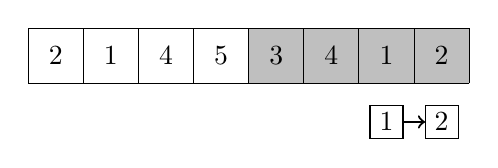
\begin{tikzpicture}[scale=0.7]
\fill[color=lightgray] (4,0) rectangle (8,1);
\draw (0,0) grid (8,1);

\node at (0.5,0.5) {$2$};
\node at (1.5,0.5) {$1$};
\node at (2.5,0.5) {$4$};
\node at (3.5,0.5) {$5$};
\node at (4.5,0.5) {$3$};
\node at (5.5,0.5) {$4$};
\node at (6.5,0.5) {$1$};
\node at (7.5,0.5) {$2$};

\draw (6.2,0.2-1.2) rectangle (6.8,0.8-1.2);
\draw (7.2,0.2-1.2) rectangle (7.8,0.8-1.2);

\node at (6.5,0.5-1.2) {$1$};
\node at (7.5,0.5-1.2) {$2$};

\draw[->,thick] (6.8,0.5-1.2) -- (7.2,0.5-1.2);
\end{tikzpicture}
\end{center}

Since each array element
is added to the queue exactly once and
removed from the queue at most once,
the algorithm works in $O(n)$ time.



